\documentclass[11pt,professionalfonts]{article}


\usepackage{amsmath,amssymb,amsthm}
\usepackage{graphics,graphicx}
\usepackage{longfbox}
\usepackage{float}
\usepackage{setspace}

\usepackage{xepersian}
\settextfont{XB Niloofar.ttf}

\title{پروژه‌های درس پردازش تصویر}
\author{مهدی جلیلی}
\parskip=0.75cm
\linespread{1.2}
\begin{document}
	\maketitle
	
	\begin{center}
		\lfbox[border-width=1pt,padding={8pt,8pt}]{\text{\Huge پروژه‌ها}}
	\end{center}
	
	\fbox{\text{سوال اول}}
	
	برای هر تصویری که دوربین عکاسی توسط لنز می‌گیرد، یک لایه‌ی بایر 
	\text{(Bayer)}
	در حافظه‌ی دستگاه ذخیره می‌شود. یکی از روش‌های ساخت تصویر رنگی
	\text{(RGB)}
	از تصویر موزاییکی یا بایری استفاده از درونیابی دوخطی است:
	\begin{figure}[H]
		\centering
		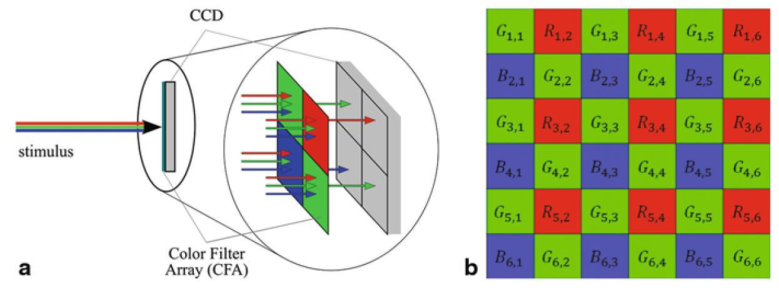
\includegraphics[width=0.95\linewidth]{Files/Bayer.png}
		\label{fig:bayer}
	\end{figure}
	برای بدست آوردن شدت رنگ متناظر کانال با توجه به نوع کانال مرکزی می‌توان محاسبات زیر را داشت:
	
	\begin{itemize}
		\item 
		\textbf{مرکز کانال قرمز:}
		\begin{align*}
			\text{if}\, R_{n,n}\, \text{center}:\Rightarrow &G_{n,n} = \frac{1}{4}(G_{n,n-1}+G_{n,n+1}+G_{n-1,n}+G_{n+1,n})\\
			& B_{n,n} = \frac{1}{4}(B_{n-1,n-1}+B_{n+1,n+1}+B_{n-1,n+1}+B_{n+1,n-1}).
		\end{align*}
		\item 
		\textbf{مرکز کانال آبی:}
		\begin{align*}
			\text{if}\, B_{n,n}\, \text{center}:\Rightarrow &G_{n,n} = \frac{1}{4}(G_{n,n-1}+G_{n,n+1}+G_{n-1,n}+G_{n+1,n})\\
			& R_{n,n} = \frac{1}{4}(R_{n-1,n-1}+R_{n+1,n+1}+R_{n-1,n+1}+R_{n+1,n-1}).
		\end{align*}
		\item 
		\textbf{مرکز کانال سبز:}
		با توجه به تعاریف بالا همسایه‌های پیکسل سبز را میانگین بگیرید.
	\end{itemize}
	تصویر بایری را که برای پروژه انتخاب شده را ابتدا آنالیز کنید و به صورت مناسب نمایش دهید. سپس تصویر را به حالت رنگی تبدیل کرده و نمایش دهید. سپس نتیجه حاصل را با تصویر رنگی واقعی مقایسه کنید و توضیح دهید چه پدیده‌هایی در تصویر تبدیل شده موجود است. برای افزایش عملکرد تبدیل تصویر بایری به رنگی چه روشی پیشنهاد می‌کنید. در نهایت تابعی برای تبدیل تصاویر رنگی به تصاویر بایری ارائه دهید (با مثال).
	
	
	\fbox{سوال دوم}
	
	در نویز زدایی تصاویر مشخصه‌ی مقدار 
	\text{PSNR}
	عملکرد نویز زدایی را نشان می‌دهد:
	\begin{align*}
		PSNR &= 10\log_{10}\bigg(\frac{Max^{2}}{MSE}\bigg),\\
		MSE &= \frac{1}{M\times N}\sum\limits_{i=1}^{N}\sum\limits_{j=1}^{M} (Y(i,j)-X(i,j))^{2}
	\end{align*}
	که در آن 
	$X$
	تصویر اصلی بدون نویز
	$Y$
	تصویر فیلتر شده و 
	$Max$
	ماکزیمم شدت ممکن برای تصویر است.
	
	
	یک تصویر نویزی بسازید با دو نوع نویز نمک و فلفل و گاوسی و سپس توسط فیلترهای میانگین و گاوسی به صورت زیر نویز زدایی انجام دهید.
	
	\begin{align*}
		Y(i,j) = \frac{\sum\limits_{k,l}I(k,l)w(i,j,k,l)}{\sum\limits_{k,l}w(i,j,k,l)}
	\end{align*}
	که در آن 
	$I$
	تصویر مورد نظر و 
	$w$
	تابع وزن می‌باشد که برای میانگین و گاوسی به صورت زیر تعریف می‌شود:
	\begin{align*}
		w(i,j,k,l)  = \frac{1}{N^{2}} \,\, \text{Mean},\quad w(i,j,k,l) = \frac{1}{\sqrt{2\pi}\sigma}e^{-\frac{(k-i)^{2}+(l-j)^{2}}{2\sigma^{2}}}\,\,\text{Gaussian}
	\end{align*}
	که در آن‌ها 
	$N$
	اندازه فیلتری است که قرار است اعمال شود. یک فیلتر جدید بسازید که تابع وزن آن به صورت زیر باشد:
	\begin{align*}
		w(i,j,k,l) = e^{-\frac{(k-i)^{2}+(l-j)^{2}}{2\sigma_c^{2}} - \frac{\|I(i,j)-I(k,l)\|^{2}}{2\sigma_s^{2}}}
	\end{align*}
	تصاویر نویزی را با این فیلترها فیلتر کرده و تفاوت‌ها و فواید روش‌ها را توضیح دهید و برای نشان دادن خطای روش‌ها از مشخصه 
	\text{PSNR}
	استفاده نمایید.
	
	
	\fbox{سوال سوم}
	
	همبستگی-متقاطع بین یک تصویر مانند 
	$f$
	و یک نمونه
	$g$
	به صورت زیر محاسبه می‌شود:
	\begin{align*}
		(g ** f)[m,n]=\sum_{i=-\infty}^\infty\sum_{j=-\infty}^\infty g[i,j]\cdot f[m + i,n + j]
	\end{align*}
	
	فرض کنید شما در یک فروشگاه مواد غذایی کارمند هستید. یکی از وظایف شما این است که به صورت دوره ای قفسه ها را بررسی کنید و هر زمان که اقلام فروخته شده ای وجود دارد، آنها را ذخیره کنید. شما از این کار پرزحمت خسته شدید و تصمیم گرفتید یک سیستم بینایی کامپیوتری بسازید که اقلام موجود در قفسه را ردیابی کند. با استفاده از همبستگی-متقاطع این فرایند را انجام دهید.
	
	تابعی بسازید که عکس یک قفسه را که پر از محصول است خوانده و نمونه محصول را تشخیص داده و روی آن علامت بزند.
	
	راهنمایی:  (\begin{verbatim}
		numpy.unravel_index,
		numpy.fliplr,
		numpy.flipud
	\end{verbatim})
	
	\begin{figure}[H]
		\centering
		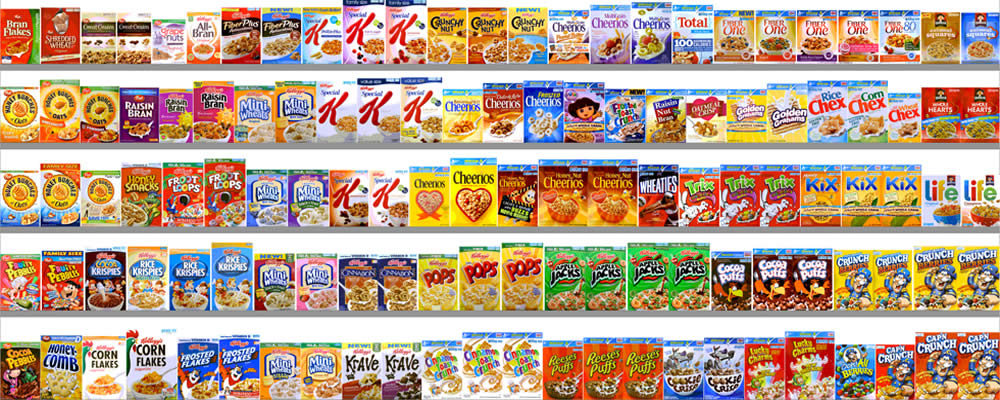
\includegraphics[width=0.7\linewidth]{Files/shelf.jpg}
		\caption{قفسه}
	\end{figure}
	\begin{figure}[H]
		\centering
		
\includegraphics[width=0.7\linewidth]{Files/template.jpg}
		\caption{نمونه}
		
	\end{figure}
	
	
\end{document}